\appendix 
\chapter{Apéndice} \label{Ch:Anex_A}

\section{Sistemas de unidades}

\section{Teoría de perturbaciones independiente del tiempo}

Consideremos un hamiltoniano sin perturbar $\Hcal_0$, con su base de autoestados (ortonormales), $\phi_a$ y sus correspondientes autovalores $E_a$:

\begin{equation}
    \Hcal_0 \phi_a = E_a \phi_a \tquad \langle \phi_a | \phi_b \rangle = \delta_{ab}
    \label{Ec:A-02-01}
\end{equation}
Ahora supongamos que existe un término pequeño $\delta \Hcal$ del Hamiltoniano, proporcional a un parámetro pequeño $\varepsilon$. En ese caso los valores de la energía sufren una transformación $E_a \rightarrow E_a + \delta E_a$, con un cambio en su correspondiente autoestado $\phi_a \rightarrow \phi_a + \delta \phi_a$, donde $\delta E_a$ y $\delta \phi_a$ están dados por una serie de potencias de $\varepsilon$:

\begin{equation}
    \delta E_a = \delta_1 E_a + \delta_2 E_a + \ldots \tquad \delta \phi_a = \delta_1 \phi_a + \delta_2 + \ldots 
\end{equation}
con el valor de $\delta_n E_a$ y $\delta_n \phi_a$ proporcioanl a $ \varepsilon^n$. La ecuación de Schrödinger puede ser expresada como:

\begin{equation}
    \parentesis{\Hcal_0 + \delta \Hcal} \parentesis{\phi_a + \delta \phi_a} = \parentesis{E_a + \delta E_a} \parentesis{\phi_a + \delta \phi_a}
\end{equation}
de tal modo que:

\begin{equation}
    \Hcal_0  \phi_a + \Hcal_0 \phi_a + \delta H \phi_a = E_a \phi_a + E_a \delta \phi_a + \delta E_a \phi_a + \delta E_a \delta \phi_a \label{Ec:A-02-04}
\end{equation}
Dado que $\Hcal_0 \phi_a = E_a \phi_a$ (\ref{Ec:A-02-01}) la eliminamos en ambos lados:
 
\begin{equation}
    \Hcal_0 \phi_a + \delta H \phi_a = E_a \phi_a + E_a \delta \phi_a + \delta E_a \phi_a  \label{Ec:A-02-05}
\end{equation}

\subsection{Primer orden}

Para calcular la perturbación de primer orden nos tenemos que fijar cuales son los términos que van con $\varepsilon$. Aquellas que vayan con $\varepsilon^2$ pertenecerán a lo que llamamos perturbación de segundo orden (apartado \ref{Subsec:A-02-02}), de tal modo que $\delta\Hcal\delta\phi_a$ y $\delta E_a\delta\phi_a$ no vamos a tenerlas en cuenta. Así, para los términos de primer orden $\varepsilon$:

\begin{equation}
    \Hcal_0 \delta_1 \phi_a + \delta \Hcal \phi_a = E_a \delta_1 \phi_a + \delta_1 E_a \phi_a \label{Ec:A-02-06}
\end{equation}
Para encontrar $\delta_1 E_a$ tenemos que realizar el producto escalar en la ecuación anterior con $\phi_a$:

\begin{equation}
    \langle \phi_a | \Hcal_0 \delta_1 \phi_a \rangle + \langle \phi_a | \delta \Hcal \phi_a \rangle = E_a \langle \phi_a |\delta_1 \phi_a \rangle + \delta_1 E_a \langle \phi_a |\phi_a \rangle
\end{equation}
Dado que $\Hcal$ es hermítico, tenemos que $\langle \phi_a |\Hcal_0 \delta_1 \phi_a\rangle = \langle \Hcal_0 \phi_a |\delta_1 \phi_a\rangle = E_a \langle \phi_a |\delta_1 \phi_a \rangle $, con lo cual se cancelan los términos.

\begin{equation}
    \delta_1 E_a = \langle \phi_a |\delta \Hcal |\phi_a\rangle  \label{Ec:A-02-08}
\end{equation}
Sin embargo, este procedimiento es solo aplicable a estados no degenerados. Para ver el porqué, tendremos que calcular el cambio de una autofunción producido por una perturbación. Tomemos entonces el producto escalar de (\ref{Ec:A-02-06}) con el autoestado de la función del estado fundamental.

\begin{equation*}
    \langle |\Hcal_0 \delta_1 \phi_a \rangle + \langle \phi_b | \delta \Hcal \phi_a\rangle = E_a \langle \phi_b |\delta_1 \phi_a \rangle + \delta_1 E_a \langle \phi_a | \phi_n \rangle
\end{equation*}
\begin{equation}
\langle \phi_b |\delta \Hcal |\phi_a \rangle = (E_a - E_b) \langle |\delta_1 \phi_a\rangle
\end{equation}
Para $a=b$ tendríamos que esta ecuación es igual a (\ref{Ec:A-02-08}). Lo que ahora conocemos, a diferencia de antes, es que

\begin{equation}
    \langle \phi_b |\delta \Hcal |\phi_a \rangle = (E_a - E_b) \langle \phi_b |\delta_1 \phi_a \rangle, \tquad \text{para}  \ a \neq b
\end{equation}
Ahora el problema es claro: si existen dos estados con $\phi_b \neq \phi_a$ tal que $E_b = E_a$, entonces la ecuación anterior es inconsistente a menos que $\langle \phi_b | \delta \Hcal |\phi_a\rangle$ sea coer, lo cual no suele ser el caso.

\subsubsection{Estados no degenerados}

Primero vamos a estudiar el caso mas sencillo posible: el estado no degenerado. En otras palabras: cada estado tiene su propia energía, diferente a cualquier otro estado. En este caso podemos escribir:

\begin{equation}
    \langle \phi_b |\delta_1 \phi_a \rangle = \frac{\langle \phi_b |\delta \Hcal |\phi_a \rangle}{(E_a - E_b)}, \tquad \text{para}  \ a \neq b \label{Ec:A-02-11}
\end{equation}
Ahora bien, ¿Qué pasa con el componente de $\delta_1 \phi_a$ proyecto sobre $\delta_a$ dado por $\langle \phi_a |\delta_1 \phi_a \rangle$? Para encontar el valor necesitamos imponer la condición de que $\phi_a + \delta_1 \phi_a$ está normalizada, esto es:

\begin{equation}
    1 = \langle \phi_a + \delta_1 \phi_a | \phi_a + \delta_1 \phi_a \rangle = 1+ \langle \phi_a |\delta_1 \phi_a \rangle + \langle \phi_a | \phi_a \rangle + \Ocal (\varepsilon^2)
\end{equation}
De lo cual se deduce la condición de que 

\begin{equation}
     \Real \parentesis{\langle \phi_a |\delta_1 \phi_a \rangle }=0
\end{equation}
No hay que imponer nada a la parte imaginaria del producto $\langle \phi_a | \delta_1 \phi_a \rangle $, y dado que este valor, en realdiad, lo podemos elegir libremente, ya que solo representa la elección de fase del vector. En partircular elegimos que $\langle \phi_a | \delta_1 \phi_a \rangle $ sea real, de tal modo que la condición de noramlización es tan sencilla como

\begin{equation}
    \langle \phi_a |\delta_1 \phi_a \rangle = 0
\end{equation}
Volviendo a la ecuación (\ref{Ec:A-02-11}) y usamos que

\begin{equation}
    \delta_1 \phi_a = \sum_b |\phi_b \rangle \langle \phi_b | \delta_1 \phi_a \rangle = \sum_{b \neq a} \frac{\langle \phi_b |\delta \Hcal |\phi_a \rangle}{(E_a-E_b)} |\phi_b \rangle \label{Ec:A-02-16}
\end{equation}
de tal modo que la \textit{perturbación de primer orden} para $\phi_a$ es:

\begin{equation}
    \delta_1 \phi_a = \sum_{b\neq a} \frac{\langle \phi_b |\delta \Hcal |\phi_b \rangle}{(E_a - E_b)}|\phi_b \rangle
\end{equation}

\subsubsection{Estados degenerados}

Supongamos que hay un número de estados $\phi_{a_1}, \phi_{a_2},\ldots, \phi_{a_n}$, todos con la misma energía $E_a$.  En este caso la ecuación (\ref{Ec:A-02-16}) debe ser dividida en dos partes, uno para las la suma de los estados con energías diferentes y otro para los estados con la misma energía, tal que:

\begin{eqnarray}
	\delta_1 \phi_a = \sum_{c:E_c\neq E_a}\frac{\langle \phi_c | \delta \Hcal | \phi_a \rangle}{(E_a-E_c)} |\phi_c\rangle + \sum_{b:E_b = E_a} |\phi_b \rangle \langle \phi_b | \delta_1 \phi_a \rangle
\end{eqnarray}

% Falta mucho texto

\subsection{Segundo orden} \label{Subsec:A-02-02}

Vamos a calcular ahora el cambio de los valores de la energía debido a una perturbación $\delta \Hcal$ pero ahora para los términos de segundo orden. Las perturbaciones de segundo orden son especialmente importantes cuando los términos de primer orden son nulos, como puede ocurrir con el \textit{efecto Stark} para los estados del hidrógeno $1s_{1/2},2p_{3/2}$... y para otros átomos. 

Podemos calcular la perturbación de segundo orden debidas solo al término $\delta_1 \Hcal$ (que contiene un solo $\varepsilon$), sin embargo con un pequeño esfuerzo podemos incluir el término $\delta_2 \Hcal$ ($\varepsilon^2$) de tal modo que

\begin{eqnarray}
	\Hcal= \Hcal_0 +\delta_1 \Hcal + \delta_2 \Hcal 
\end{eqnarray}
Volviendo a la ecuación original (\ref{Ec:A-02-04}) podemos ver que, los términos de segundo orden a ambos lados son:

\begin{eqnarray}
	\Hcal_0 \delta_2 \phi_a + \delta_2 \Hcal \phi_a + \delta_1 \Hcal \delta_1 \phi_a = E_a \delta_2 \phi_a + \delta_2 E_a \phi_a + \delta_1 E_a \delta_1 \phi_a
	\label{Ec:A-02-21}
\end{eqnarray}

\subsubsection{Caso no degenerado}

Vamos a calcular en primera instancia el caso no degenerado, en el que los estados no tienen las mismas energías sin perturbar. Para encontrar los términos de segundo orden, debemos ver que:

\begin{eqnarray*}
	\langle \phi_a | \Hcal_0 | \delta_2 \phi_a \rangle + \langle \phi_a |\delta_2 \Hcal | \phi_a \rangle + \langle \phi_a |\delta_1 \Hcal | \delta_1 \phi_a \rangle = E_a \langle \phi_a |\delta_2 \phi_a \rangle + \delta_2 E_a + \delta_1 E_a \langle \phi_a |\delta_1 \phi_a \rangle 
\end{eqnarray*}
Dado que $\Hcal_0$ es hermítico, tenemos que los términos $\langle \phi_a | \Hcal_0 |\delta_2 \phi_a \rangle = E_a \langle \phi_a |\delta_2 \phi_a\rangle$ se cancelan, por lo que la ecuación queda de la forma

\begin{eqnarray}	
	\langle  \phi_a |\delta_2 \Hcal |\phi_a \rangle + \langle \phi_a |\delta_1 \Hcal | \delta_1 \phi_a \rangle =   \delta_2 E_a + \delta_1 E_a \langle \phi_a |\delta_1 \phi_a \rangle 
\end{eqnarray}
Elegimos normalizar la fase de los vectores perturbados de tal manera que $\langle \phi_a |\delta_1 \phi_a\rangle = 0$ (como antes), de esta manera tenemos que:

\begin{eqnarray}
	\delta_2 E_a = \langle \phi_a |\delta_2 \Hcal |\phi_a \rangle + \langle \phi_a |\delta_1 \Hcal |\delta_1 \phi_a \rangle
\end{eqnarray}
El segundo término de la matriz de la derecha puede ser calculado con la perturbación de primer orden:

\begin{eqnarray}
	\delta_1 \phi_a = \sum_{b\neq a} \frac{\langle \phi_b | \delta_1 \Hcal |\phi_a\rangle}{(E_a-E_b)} |\phi_b\rangle
\end{eqnarray}
Así la perturbación de segundo orden viene dada por


\begin{eqnarray}
	\delta_2 E_a = \sum_{b\neq a} \frac{\langle \phi_b | \delta_1 \Hcal |\phi_a \rangle |^2}{(E_a - E_b)} + \langle \phi_a |\delta_2 \Hcal |\phi_a \rangle
\end{eqnarray}
Cuando uno dice que la perturbación de la energía se produce por la emisión y reabosrción de una partícula virtual, como el la perturbación de Lamb (en este caso la partícula es un fotón absorbido por un electrón del átomo de hidrógeno), nos quiere decir que $\delta_2 E_a$ (o una corrección más alta) recibe una contribución importante corrección por parte del estado $\phi_b$. Además si $\phi_a$ es el estado con menor energía (estado fundamental) tenemos que la perturbación de segundo orden es siempre negativa (ya que $E_a-E_b<0$).

%Para calcular los valores de la perturbación de segundo orden $\delta_2 \phi_a$ necesitamos tomar el producto escalar de la función (\ref{Ec:A-02-21}) para la cual $\phi_b$ verifique $b\neq a$, e imponer la condición de que $\phi_a + \delta_1 \phi_a + \delta_2 \phi_a + \ldots$ tiene un valor unitario para encontrar % No se que coño quiere decir aquí

\subsubsection{Caso degenerado}

El en caso degenerado algunos estados en los que estamos interesados tienen la misma energía de perturbación, para la cual podemos encontrar que las energías perturbadas vienen dadas por:

\begin{eqnarray}
	\delta_2 E_a = \sum_{c:E_c\neq E_a} \frac{\langle \phi_a|\delta_1 \Hcal |\phi_c\rangle |^2}{(E_a-E_c)} + \langle \phi_a |\delta_2 \Hcal |\phi_a \rangle
\end{eqnarray}

\section[Regla de Oro de Fermi]{Teoría de perturbaciones dependiente del tiempo. Regla de oro de Fermi}

Supongamos que $\phi_k (\xn,t)$ son soluciones (convenientemente normalizadas y ortogonales) de la ecuación de Schrödinger para el hamiltoniano sin perturbar e independiente del tiempo $\Hcal_0$, de tal modo que

\begin{eqnarray}
	\Hcal_0 \phi_k = E_k \phi_k \tquad \langle \phi_j |\phi_k \rangle = \delta_{jk}
\end{eqnarray}
Ahora aplicamos una perturbación en el Hamiltoniano dependiente del tiempo mucho mas pequeño que el Hamiltoniano $\Hcal_0$ tal que $\Hcal=\Hcal_0 + V(\xn,t)$. Así:

\begin{eqnarray}
	i \hbar \derivadas{\psi}{t} = \ccorchetes{\Hcal_0 + V(\xn,t)}\psi
\end{eqnarray}
Si consideramos a los $\phi_k$ unos autoestados válidos del sistema perturbado, está claro que cualquier estado (representado por $\psi(\xn,t)$, un ``estado genérico'') puede describirse como 

\begin{eqnarray}
	\psi(\xn,t) = \sum_k c_k(t) \phi_k (\xn) e^{-iE_kt/\hbar}
\end{eqnarray}
Nótese que los coeficientes $c_k(t)$ son dependientes del tiempo, lo cual conduce a la posibilidad de que ocurran transiciones entre estados. Introduciendo esto en las ecuaciones anteriores nos dejan una serie de ecuaciones diferenciales:

\begin{eqnarray}
	i \hbar \sum_k \derivadas{c_k}{t} \phi_k e^{-iE_k t/\hbar} = \sum_k Vc_k (t) \phi_k e^{-iE_kt/\hbar} \label{Ec:A-03-04}
\end{eqnarray}

Asumamos ahora que el sistema en el instante $t=0$ era $\phi_i \equiv |i\rangle$. Los coeficientes para $t=0$ venían dados por $c_k (0)=\delta_{ik}$. Asumiento un Hamiltinano suficientemente pequeño de tal modo que los coeficientes, como \textit{primera aproximación}, cumplieran que $c_i(t)\approx 1$ y $c_{k\neq i}(t) \approx 0$, tendríamos que la ecuación (\ref{Ec:A-03-04}) podría escribirse como

\begin{eqnarray}
	i \hbar \sum_k \derivadas{c_k}{t} \phi_k e^{-iE_kt/\hbar} \approx V\phi_i e^{-iE_it/\hbar}
\end{eqnarray}
Estamos interesados en calcular la \textit{probabilidad de transición} del estado inicial $|i\rangle$ a un estado final particular $|f\rangle$, ya que está relacionada con la derivada $\D c_f / \D t$ (siendo $f$ un estado cualquiera), lo cual puede verse fácilmente multiplicando la ecuación anterior por $\langle f | \equiv \phi_f^*$ e integrando, de tal modo que

\begin{eqnarray*}
	i \hbar \sum_k \derivadas{c_k}{t} e^{-iE_kt/\hbar} \int \phi_f^*  \D \xn  = \phi_i e^{-iE_it/\hbar}\int \phi_f^* V \phi_i \D \xn
\end{eqnarray*}
y como $\langle i | f\rangle=\delta_{fi}$ (esto es $\int \phi_f^* \phi_i \D \xn=\delta_{fi}$), pasando todos los términos menos la derivada a la derecha:

\begin{eqnarray}
	  \derivadas{c_f}{t} = -\frac{i}{\hbar} e^{-i(E_i-E_k)t/\hbar}\int \phi_f^* V \phi_i \D \xn
\end{eqnarray}
Como dijimos antes, la derivada está relacionada con el término de transición $T_{fi}$, que pertenece a la \textit{matriz de transición} $T$. Integrando podemos ver que

\begin{eqnarray}
	T_{fi} = \langle \phi_f | V |\phi_i \rangle + \sum_{k\neq i} \frac{\langle \phi_f |V|\phi_k \rangle \langle \phi_k |V|\phi_i\rangle }{(E_k - E_i)}
\end{eqnarray}
de tal modo que la ecuación diferencial nos queda como:

\begin{eqnarray}
	\derivadas{c_f}{t} = - \frac{i}{\hbar} T_{fi} e^{-i(E_i-E_k)t/\hbar}
\end{eqnarray} 

\subsection{Regla de Oro de Fermi}

Sea $P_{fi}$ la probabilidad de transición del estado $|f\rangle$ en el instante $T$:
\begin{eqnarray}
	P_{fi} = c_f^*(T) c_f(T)
\end{eqnarray}
El resultado de la integral nos lleva directamente a que

\begin{eqnarray}
	P_{fi} = \frac{4|T_{fi}|^2}{(E_f-E_i)^2} \sin^2 \ccorchetes{\frac{(E_f-E_i)T}{2\hbar}}
\end{eqnarray}

Denotando la \textit{probabilidad de transición por unidad de tiempo} $\Gamma_{fi}$ del estado $|i\rangle$ a $|f\rangle$, de tal modo que

\begin{eqnarray}
	\Gamma_{fi} = \derivadas{P_{fi}}{T}
\end{eqnarray}
de lo cual se deduce que 

\begin{eqnarray}
	\Gamma_{fi} = \frac{2 |T_{fi}|^2}{\hbar(E_f-E_i)} \sin \ccorchetes{\frac{(E_f-E-i)T}{\hbar}}
\end{eqnarray}
Dado que nos interesa ver que pasa cuando $T\rightarrow \infty$, tenemos que solo obtendremos valores interesantes cuando $E_f=E_i$ (ya que tendremos $ \sin(0)/0$, esto es, 1), por lo que si $T\rightarrow \infty$, tenemos que

\begin{eqnarray}
	\Gamma_{fi} = \frac{2\pi}{\hbar} |T_{fi}|^2 \delta (E_f -E_i)
\end{eqnarray}
que la \textbf{regla de oro de Fermi}. Otra manera de expresar la regla de oro de Fermi, muy interesante, tiene que ver con la \textit{transición al estado final $|i\rangle$ por unidad de tiempo}, esto es, la suma de todas las transiciones que producen $i$. Para computar esto tendríamos que hacer un sumatorio, pero suponiento una densidad de estados energéticos $\rho(E)$ ($\rho(E)\D E$ es el número de estados que hay entre $E$ y $E+\D E$), la probabilidad de transición total es la integral en todo el espectro de energías $E_f$, pero como hay una delta de Dirac, finalmente resulta que:

\begin{eqnarray}
	\Gamma_i = \frac{2\pi}{\hbar} |T_{fi}|^2 \rho (E_i)
\end{eqnarray}


\section{Métodos variacionales}

Vamos a ver como la ecuación de Schrödinger puede ser derivada del método variacional, par amás tarde ver como nos permite obtener soluciones aproximadas a la ecuación de Schrödinger. Para calcular la ecuación de Schrödinger tenemos que encontrar el extremo del funcional $I=\langle \psi |\Hcal|\psi\rangle $ bajo la conidición de que $\langle \psi | \psi \rangle= 1$. En otras palabras, vamos a buscar cual es la ecuación de Euler-Lagrange que debe satisfacer $\psi$ para que $\delta I = 0$. Esto se puede hacer exigiendo que

\begin{eqnarray}
	\delta \ccorchetes{\langle \psi | \Hcal |\psi \rangle - \lambda \langle \psi |\psi \rangle = 0} = 0
\end{eqnarray} 
donde $\lambda$ es el multiplicador de Langrande. Podemos escribir:

\begin{eqnarray}
	\delta \ccorchetes{\langle \psi |\Hcal |\psi \rangle - \lambda \langle \psi |\psi \rangle } = \langle \delta \psi | (\Hcal - \lambda) | \psi \rangle + \langle \psi | (\Hcal - \lambda) |\delta \psi \rangle = 0
\end{eqnarray}
Aunque $|\delta \psi \rangle$ y $\langle \delta \psi |$ no son independientes, vamos a ver que si $\delta \psi = \delta u + i \delta v$, esto nos lleva a que

\begin{equation}
	\langle \delta \psi |\Hcal - \lambda |\psi \rangle + \langle \psi |(\Hcal - \lambda) |\delta \psi \rangle  = \langle \delta u | (\Hcal - \lambda) | \psi + \psi^* \rangle - i \langle \delta v |(\Hcal - \lambda ) |\psi - \psi^* \rangle    = 0
\end{equation}
para cualquier $\delta u $ y $\delta v$ (que son independientes). Entonces las ecuaciones de Euler-Lagrange para este problema variacional son:

\begin{eqnarray}
	(\Hcal - \lambda) |\psi + \psi^* \rangle = 0 \tquad (\Hcal - \lambda) |\psi - \psi^*\rangle = 0
\end{eqnarray}
de lo cual obtenemos otras ecuaciones:

\begin{eqnarray}
	(\Hcal - \lambda) |\psi \rangle = 0 \tquad (\Hcal - \lambda) |\psi^*\rangle = 0
\end{eqnarray}
Estas dos ecuaciones son equivalentes a la ecuación de Schrödinger $(\Hcal - E) |\psi\rangle$ donde el multiplicador de Lagrange debe ser un autoestado del Hamiltoniano. Consecuentemente, cualquier función $\psi$ para el que el funcional $I=\langle \psi | \Hcal | \psi \rangle $ es estacionario será una autofunción de $\Hcal$ con autovalor $E$. De otra forma, si $\psi$ es un autoestado de $\Hcal$ siendo $E$ su autovalor correspondiente, $
I$ será estacionario.

El método variacional, como vamos a ver, nos permite calcular soluciones de la ecuación de Schrödinger. El método se basa en probar una ecuación $\psi$ que servirá como una solución aproximada. Definiendo la energía $E$ como

\begin{eqnarray}
	E = \frac{\langle \psi |\Hcal |\psi \rangle}{\langle \psi |\psi \rangle}
\end{eqnarray}
Sea $\psi_k$ ser un autofunción de $\Hcal$ con autovalor $E_k$. Entonces:

\begin{eqnarray}
	E-E_k = \frac{\langle \psi |(\Hcal-E_k)|\psi \rangle}{\langle \psi |\psi \rangle}
\end{eqnarray}
Si ahora asumimos que la diferencia entre $\psi$ y $\psi_k$ viene dada por un término $\delta\psi$ muy pequeña tal que

\begin{eqnarray}
	\psi = \psi_k + \delta \psi \tquad \langle \psi_k |\psi \rangle = 0
\end{eqnarray}
De este modo tenemos que:

\begin{eqnarray}
	E-E_k =  \frac{\langle \psi_k + \delta \psi |\Hcal |\psi_k + \delta \psi \rangle}{\langle \psi |\psi \rangle} =  \frac{\langle \delta \psi |\Hcal |\delta \psi \rangle}{\langle \psi |\psi \rangle}
\end{eqnarray}
Esto nos dice que la diferencia entre el valor $E$ y el autovalor real $E_k$ varia cuadráticamente con $\delta \psi$. La perturbación de $E$ más pequeña es de segundo orden, por lo que el término de primer orden $\delta E$ debe ser nulo. Esto es el llamado \textbf{principio variacional}, que dice que la mejor aproximación del autovalor $E_k$ se obtiene cambiando $\psi$ (o de los parámetros de los que dependa $\psi$), de tal modo que $\delta E=0$ se satisfaga. \\


\section{Momento angular y espín}

Las leyes de la naturaleza no deberían depender de como este orientado nuestro laboratorio. Se espera entonces que nuestras teorías sean invariante bajo rotaciones. Esta invariancia bajo rotaciones nos lleva a la existencia de una cantidad conservada, el momento angular. En tres dimensiones es muy conveniente expresar el momento angular $J_{ij}$, que es la cantidad conservada al rotar el plano $ij$, como $J_{k}$, esto es, la dirección perpendicular al plano $ij$. En este caso tenemos que se cumple para $i,j,k=1,2,3$ que 

\begin{eqnarray}
	J_1 \equiv J_{23} \quad J_2 \equiv J_{31} \quad J_3 \equiv J_{12}
\end{eqnarray}
o de un modo más compacto:

\begin{eqnarray}
	J_k \equiv \sum_k \frac{1}{2} \epsilon_{ijk} J_{ij} \quad J_{ij} = \sum_k \epsilon_{ijk} J_k
\end{eqnarray}
Se puede demostrar que la conmutación del vector $\Jn$ con cualquier otro vector $\Vn$ verifica que

\begin{eqnarray}
	[J_i,,V_j] = i\hbar \sum_k \epsilon_{ijk} V_k
\end{eqnarray}
De hecho, un \textit{podemos definir un operador vector como aquel que verifica las relaciones de conmutación con los generadores de rotaciones espaciales}. Un operador escalar conmuta con dichos generadores de la forma $[J_i,S]=0$. Además, se verifica que las relaciones entre componentes de $\Jn$

\begin{eqnarray}
	[J_i,J_j] = i\hbar \sum_k \epsilon_{ijk} J_k
\end{eqnarray}
Usando estas relaciones de conmutación es posible obtener los autovalores de $\Jn^2$ y $J_3$, así como la acción de $\Jn$ sobre los autovectores de dichos operadores (recordemos que $\Jn^2$ y $J_3$ conmutan como 0, por lo que son mutuamente diagonalizables). Los autovalores de $\Jn^2$ y $J_3$ se denotan por los números cuánticos $j$ y $m$, con $j$ como un \textit{\textbf{enerto o semientero}} y $m$ teniendo valores de $-j$ a $j$. Denotando los autoestados como $|jm\rangle$, tenemos que:

\begin{eqnarray}
	J_3 |jm\rangle = \hbar m |jm\rangle \tquad \Jn^2 |jm\rangle = \hbar^2 j(j+1) |jm\rangle \tquad m=-j,-j+1,\ldots,j
\end{eqnarray}
En general podemos expresar $\Jn$ como la suma de dos términos, tal que

\begin{eqnarray}
	\Jn = \Ln + \Sn
\end{eqnarray}
a $\Ln$ lo llamamos \textit{momento angular espacial} y a $\Sn$ \textit{momento angular intrínseco} o \textit{espín}. Estos conmutan entre sí 

\begin{eqnarray}
	[S_i,L_j] = 0
\end{eqnarray}
De tal modo que se verifica

\begin{eqnarray}
	[S_i,S_j] = i \hbar \sum_k \epsilon_{ijk} S_k \tquad [L_i,L_j] = i \hbar \sum_k \epsilon_{ijk} L_k
\end{eqnarray}
Además tenemos las siguientes relaciones, sumamente importantes:

\begin{eqnarray}
J_{\pm}|jm\rangle = (J_1 \pm i J_2) |jm\rangle = \hbar \sqrt{j(j+1)-m(m\pm1)} |jm\pm1\rangle
\end{eqnarray}
De tal modo que 

\begin{eqnarray}
	J_1 = \frac{1}{2} (J_+ + J_-) \tquad J_2 = \frac{1}{2i} (J_+-J_-)
\end{eqnarray}


\subsection{Momento angular para $j=1/2,1,3/2$}

\subsection{Representaciones del operador rotación: matrices de rotación}

Consideremos un sistema de autovectores $|j,m\rangle$. Queremos encontrar los elementos del oeprador unitario $U(R)$ que nos permite implementar rotaciones espaciales en el sistema. Recordemos que el operador $U(R)$ viene dado por 

\begin{eqnarray}
	U(R) = \exp \parentesis{- \frac{i}{\hbar} \Jn \cdot \omegan}
\end{eqnarray}
La rotación se realiza alrededor de la dirección del vector $\omegan$ por un ángulo $|\omegan|$ en radianes. $[J^2,J_i]=0$, tal que $[U(R),J^2]=0$ y los elementos de matriz de $U(R)$ deben ser diagonales en $j$ tal que

\begin{eqnarray}
	\langle j',m' |U(R)|j,m\rangle \propto \delta_{j'j}
\end{eqnarray}
Para un $j$ dado, $U(R)$ el operador puede ser representado por la matriz $(2j+1)\times (2j+1)$ y denotado por $D_{m'm}^{(j)} (R)$, cuyos elementos son

\begin{eqnarray}
	D_{m'm}^{(j)} (R) \equiv \langle j,m' |U(R) | j,m\rangle
\end{eqnarray}
Estas matriz son llamadas las \textit{matrices de rotación} o \textit{matrices de Wigner}. Los vectores de rotación vienen dadas pro la ecuación

\begin{eqnarray}
	|j,m\rangle_R = U(R) |j,m\rangle = \sum_{m'} |j,m'\rangle \langle j,m'|U(R)| j,m\rangle
\end{eqnarray}
Esto nos dice directamente como obtener $|j,m\rangle_R$ en términos de los elementos de la matriz de rotación:

\begin{eqnarray}
	|j,m\rangle_R = \sum_{m'} D_{m'm}^{(j)} (R) |j,m'\rangle
\end{eqnarray}
Como ejemplo, la matriz de rotación para un sistema con $j=1/2$ viene dada por 


\begin{eqnarray}
	D^{(1/2)}(\theta,\varphi) = \begin{pmatrix}
		e^{-i\varphi/2} \cos (\theta/2)  & 	-e^{-i\varphi/2} \sin (\theta/2) \\
		e^{i\varphi/2} \sin (\theta/2) & 	e^{i\varphi/2} \cos (\theta/2)
	\end{pmatrix}
\end{eqnarray}

donde $\theta$ y $\varphi$ son los ángulos polares y azimutales propios de las coordenadas esféricas.


\subsection{Coeficientes de Clebsch-Gordan, símbolos $3j$ y $6j$}

Dos sistemas con momentos angulares $\Jn_1$ y $\Jn_2$ pueden ser considerados juntos como un sistema global de momento angular total $\Jn_3 = \Jn_1 + \Jn_2$. Existen dos bases de autofunciones de este tercer sistema, representadas por $|j_1 j_2 j_3 m_3\rangle$ y $|j_1 j_2 m_1 m_2\rangle$. Las relaciones vienen dadas por:

\begin{equation}
   |j_1 j_2 j_3 m_3 \rangle  = \sum_{m_1, m_2}  \langle j_1 j_2 m_1 m_2 | j_1 j_2 j_3 m_3 \rangle    |j_1 j_2 m_1 m_2\rangle
\end{equation}
\begin{equation}
	|j_1 j_2 m_1 m_2\rangle= \sum_{m_1, m_2} \langle j_1 j_2 m_1 m_2 | j_1 j_2 j_3 m_3 \rangle    |j_1 j_2 j_3 m_3 \rangle
\end{equation}
Los \textit{\textbf{coeficientes Clebch-Gordan} son todos reales}, por lo que 

\begin{eqnarray}
	 \langle  j_1 j_2 j_3 m_3 |  j_1 j_2 m_1 m_2\rangle  = \langle j_1 j_2 m_1 m_2 | j_1 j_2 j_3 m_3 \rangle   
\end{eqnarray}
En lugar de usar los coeficientes Clebsh-Gordan para crear los estados del momento $\Jn_3$ a partir de los momentos angulares individuales $\Jn_1$ y $\Jn_2$, es posible usar estos coeficientes para construir un estado $\Psi$ con un momento angular total cero a partir de los estados $\Psi_{j_1j_2j_3}^{m_1m_2m_3}$ con \textit{tres} momentos angulares:

\begin{eqnarray}
	\Psi = \sum_{m_1,m_2,m_3} \begin{pmatrix}
		j_1 & j_2 & j_3 \\ m_1 & m_2 & m_3
	\end{pmatrix} \Psi \Psi_{j_1j_2j_3}^{m_1m_2m_3}
\end{eqnarray}
Los coeficientes que multiplican a estos estados $\Psi_{j_1j_2j_3}^{m_1m_2m_3}$ son los llamados \textbf{símbolos 3j}, y se relacionan con los coeficientes Clebsch-Gordan de la siguiente manera

\begin{eqnarray} \begin{pmatrix}
		j_1 & j_2 & j_3 \\ m_1 & m_2 & m_3
	\end{pmatrix} = \frac{(-1)^{j_1-j_2-m_3}}{\sqrt{2j_3+1}} \langle j_1 j_2 m_1 m_2 |j_1 j_2 j_3 - m_3 \rangle
\end{eqnarray}
Debido a la simetría en la que estos 3 momentos angulares aparecen en el acoplamiento, los símbolos $3j$ son simétricos bajo permutaciones pares de columnas (cambiamos 2 columnas de posición):

\begin{eqnarray} \begin{pmatrix}
		j_1 & j_2 & j_3 \\ m_1 & m_2 & m_3
	\end{pmatrix} =  \begin{pmatrix}
	j_1 & j_3 & j_2\\ m_1 & m_3 & m_2
	\end{pmatrix} =  \begin{pmatrix}
	j_3 & j_2 & j_1 \\ m_3 & m_2 & m_1
		\end{pmatrix}
\end{eqnarray}

Mientras que bajo permutaciones impares (cambiamos las 3 columnas de posición):

\begin{eqnarray} \begin{pmatrix}
		j_1 & j_2 & j_3 \\ m_1 & m_2 & m_3
	\end{pmatrix} = (-1)^{j_1+j_2+j_3} \begin{pmatrix}
	j_3 & j_1 & j_2\\ m_3 & m_1 & m_2
	\end{pmatrix}
\end{eqnarray}
Además tenemos que:

\begin{eqnarray} \begin{pmatrix}
		j_1 & j_2 & j_3 \\ m_1 & m_2 & m_3
	\end{pmatrix} = \begin{pmatrix}
	j_2 & j_3 & j_1 \\ m_3 & m_1 & m_2
	\end{pmatrix} = \begin{pmatrix}
	j_3 & j_1 & j_2 \\ m_2 & m_3 & m_1
	\end{pmatrix}
\end{eqnarray}
Además se verifica que:
\begin{eqnarray} \begin{pmatrix}
		j_1 & j_2 & j_3 \\ m_1 & m_2 & m_3 
		\end{pmatrix}
		 = 0  \ \ \text{{\small a menos que}} \ \ m_1 + m_2 + m_3 = 0 \ \text{{\small y}}  \left. \begin{array}{c}
			j_1 + j_2 - j_3 \\
			j_1 - j_2 + j_3 \\
			-j_1 + j_2 + j_3 
		\end{array} \right\rbrace \geq 0
\end{eqnarray}
La última condición se suele denotar por $\Delta (j_1j_2j_3)$

%Cuando acoplamos 3 momentos angulares es común introducir los \textbf{símbolos 6j}, denotados por:

%\begin{eqnarray}
%	 \begin{Bmatrix}
%		j_1 & j_2 & j_3 \\ m_1 & m_2 & m_3
%	\end{Bmatrix}
%\end{eqnarray}

\begin{figure}[h!] \centering
	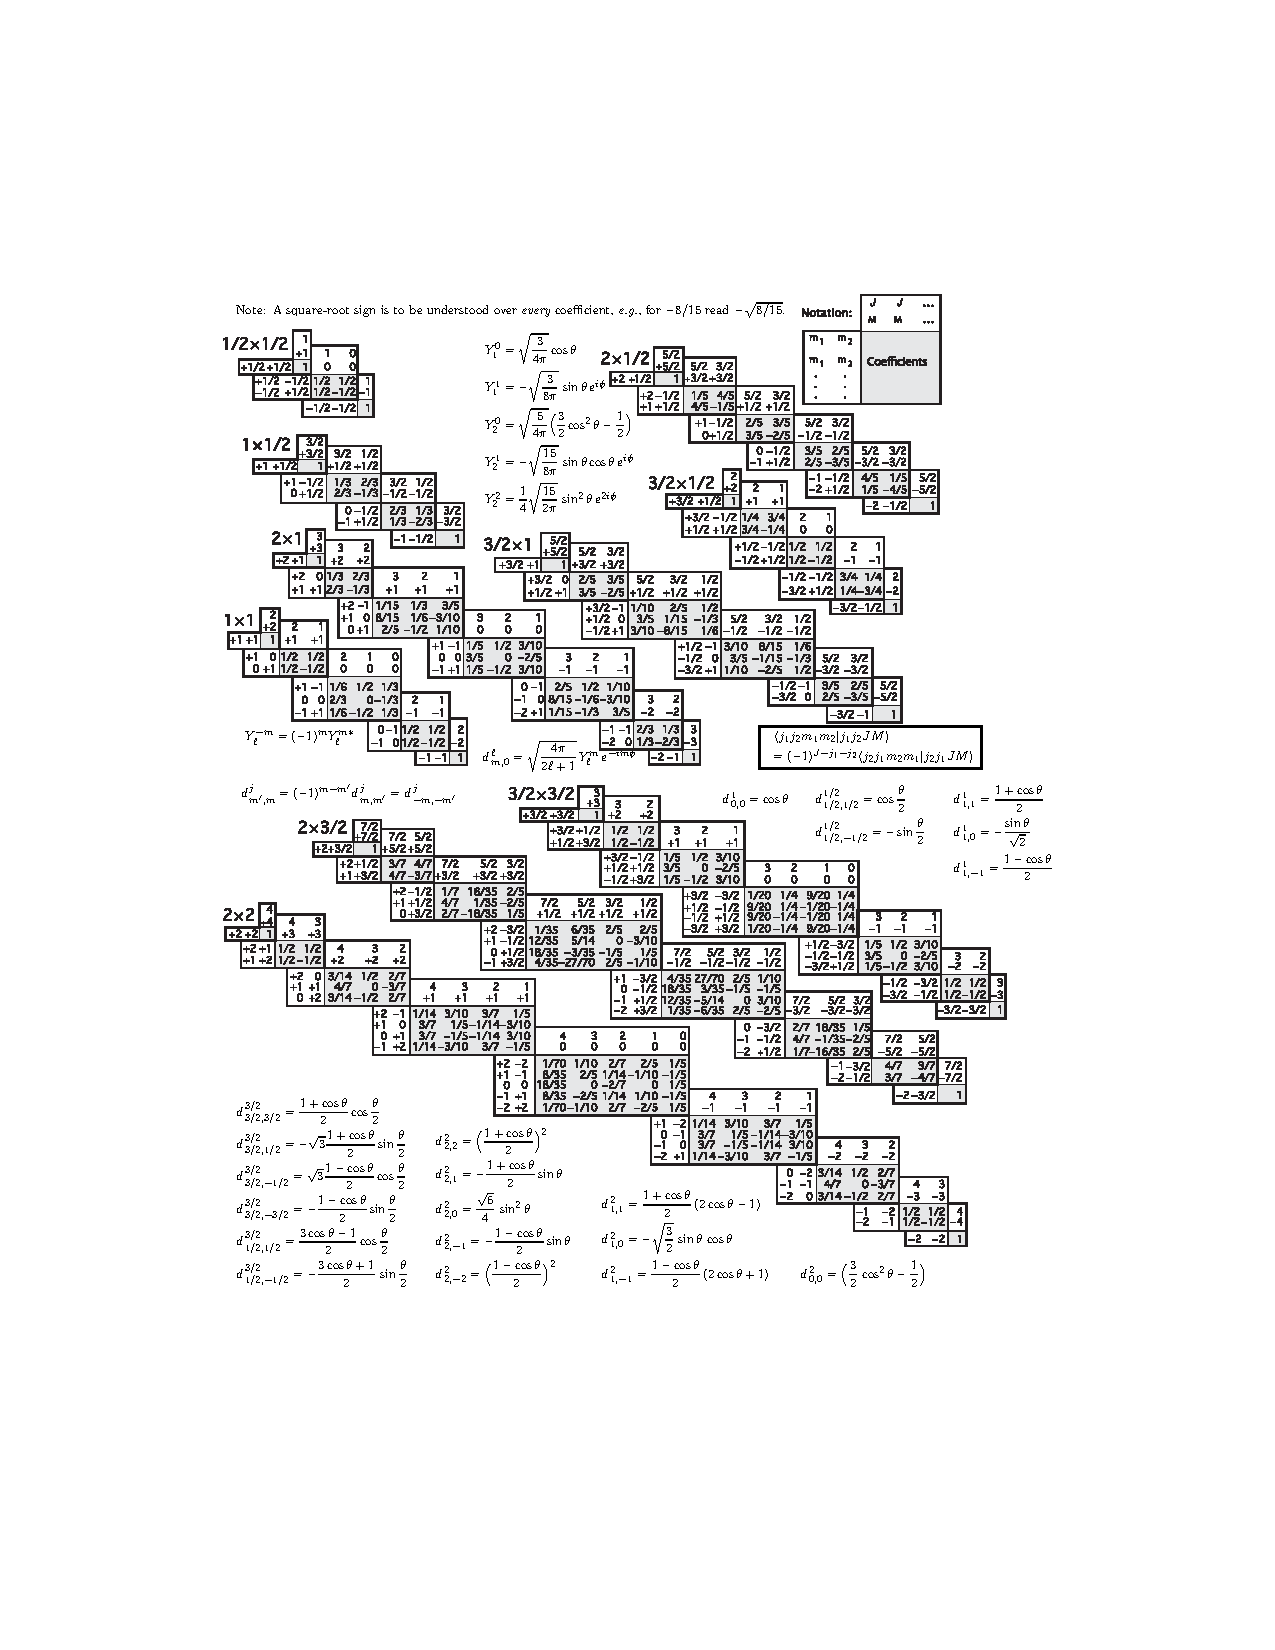
\includegraphics[width=1.\linewidth]{Cuerpo/Imagenes/A-Clebsh-Gordon.pdf}
	\caption{Coeficientes Clebsch-Gordon}
\end{figure}

\subsection{Armónicos esféricos}

Los armónicos esféricos $Y_l^m (\theta, \varphi)$ son las autofunciones del orbital momento angular orbital, y satisfacen las siguientes ecuaciones diferenciales:

\begin{equation}
    \ccorchetes{\frac{1}{\sin (\theta)} \parciales{}{\theta} \parentesis{\sin (\theta) \parciales{1}{\theta} + \frac{1}{\sin^2 (\theta)} \parciales{^2}{\varphi^2}}} Y_l^m + l(l+1) Y_l^m = 0
\end{equation}
Y vienen dadas explícitamente por:

\begin{equation}
    Y_l^m (\theta,\varphi) = (-1)^m \ccorchetes{\frac{2l+1}{4 \pi} \frac{(l-m)!}{(l+m)!}}^{1/2} P_l^m (\cos (\theta)) e^{im\varphi}
\end{equation}

Es muy usual encontrar en determinados problemas la necesidad de integrar 3 armónicos esféricos (por ejepmlo el efecto Stark lineal), para lo cual nos ayudamos de la \textbf{fórmula de Gaunt}:

\begin{multline}
	\langle \ell' m' | Y_{L}^M | \ell m \rangle \equiv  \int ( Y_{\ell'}^{m'} ) (\theta,\varphi)  Y_{L}^M  (\theta,\varphi) (Y_{\ell}^{m}) (\theta,\varphi) \D \Omega  \\ = (-1)^{m'} \sqrt{\frac{1}{4\pi} (2\ell'+1)(2L+1)(2\ell+1)} \begin{pmatrix}
	\ell' & L & \ell  \\ -m' & m & m
	\end{pmatrix}\begin{pmatrix}
	\ell' & L & \ell \\ 0 & 0 & 0
	\end{pmatrix}
\end{multline}
De las propiedades de los símbolos $3j$ se puede deducir que esta integral debe verificar, para que no sea nula, las siguientes condiciones:

\begin{itemize}
	\item $-m'+M+m=0$
	\item $\ell'+L+\ell = 2n+1$ con $n=0,1,2,3...$.
\end{itemize}
Aunque es más fácil de recordar estas condiciones de que, $\ell'$ y $m'$ dependen de las relaciones $L\oplus \ell$, tal que:

\begin{eqnarray}
	\ell'=|L-\ell|,|L-\ell|+1,\ldots,L+\ell
\end{eqnarray}
y que se debe verificar que $m'=M+m$.

\subsection{El teorema de Wigner-Eckart}

Sean los $|\Phi_j^m\rangle$ los autoestados del momento angular con autovalores $j(j+1 )\hbar^2$ y $m_j \hbar$ para $J^2$ y $J_3$ respectivamente. Recordar que

\begin{eqnarray}
    (J_1\pm iJ_2) |\Phi_j^m \rangle = \hbar \sqrt{j(j+1)-m(m\pm 1)} |\Phi_j^{m\pm 1}
\end{eqnarray}
Sea $|\Psi_j^m\rangle$ otros autoestados del momento angular. Podemos demostrar que

\begin{equation}
    \langle \Phi_j^{m+1} | \Psi_j^{m+1} \rangle = \langle \Phi_j^m |\Psi_j^m \rangle
\end{equation}
Esto demuestra que $\langle \Phi_j^m |\Psi_j^m \rangle$ es {\it independiente} de $m$. Cualquier otro elemenot de la matriz con valores de $j$ y $m$ diferentes se anulan:

\begin{equation}
    \langle \Psi_{j_3}^{m_3} | O_{j_2}^{m_2} \rangle = 0
\end{equation}
Definimos como un {\bf tensor irreducible} de rango $j$ como un conjunto de $2j+1$ operadores $O_{j}^m$  ($m=-j,-j+1,...,j$) que al aplicarle lso generadores de rotación

\begin{equation}
    [J_3,O_j^m] = \hbar m O_j^m \tquad [J_1\pm i J_2, O_j^m] = \hbar \sqrt{j(j+1)-m(m\pm 1)} O_{j}^{m\pm 1}
\end{equation}
Algunos ejemplos de tensores irreducibles son los {\it armónicos esféricos}. 

\begin{theorem}[{\bf Wigner-Eckart}]
    Sea $\langle j_i j_2 m_1 m_2 |j_1 j_2 j_3 m_3 \rangle$ es el coeficiente de Clebsch-Gordan asociado con el acoplamiento de los momentos angulares $\Jn_1$ y $\Jn_2$ que componen $\Jn_3$; y $\langle \Phi || O || \Psi\rangle$, llamada la {\it matriz irreducible elemental}, que puede depende de todo menos de las tres componentes $m_1,m_2$ y $m_3$; el teorema de Wigner-Eckart nos dice que:

    \begin{equation}
        \langle \Phi_{j_3}^{m_3} | O_{j_1}^{m_1} |\Psi_{j_2}^{m_2} \rangle = \frac{1}{2j_3+1} \langle  j_i j_2 m_1 m_2 | j_1 j_2 j_3 m_3 \rangle \langle \Phi || O || \Psi  \rangle
    \end{equation}
    El teorema de Wigner-Eckart se puede expresar de otra forma, la {\bf Formula de Landé}. Sea $\An$ un vector cualquiera y $\Jn$ un moemnto angular. Esta fórmula nos dice que:

    \begin{equation}
        \langle \Phi_{j}^{m} | \An |\Psi_{j}^{m'} \rangle = \frac{\langle \Phi_j^m |\An \cdot \Jn | \Psi_j^m\rangle }{j(j+1)\hbar^2} \langle \Phi_j^m | \Jn| \Psi_j^{m'}  \rangle
    \end{equation}
    
\end{theorem}

\section{Operadores tensoriales irreducibles}

 
